\documentclass[aspectratio=169]{beamer}
\usefonttheme{serif}
\usepackage{xeCJK}
\usepackage{fontspec}
\usepackage{graphicx}
\usepackage{listings}
\usepackage{xcolor}
\usepackage{indentfirst}
\usepackage{tikz}
\usepackage{amssymb}
\usepackage{amsthm}
\usepackage{amsmath}
\usepackage{tabularx}
\usepackage{hyperref}
\usepackage{ulem}
\usepackage{version}
\usepackage{thmtools}
\usepackage{qtree}
\usepackage{algpseudocode}
\usepackage{mathtools}
\usepackage{multicol}
\usepackage{xcolor}

\AtBeginDocument{%
    \DeclareSymbolFont{pureletters}{T1}{\mathfamilydefault}{\mddefault}{it}%
    }

\XeTeXlinebreaklocale "zh"
\XeTeXlinebreakskip = 0pt plus 1pt

\setCJKmainfont{NotoSansTC-Medium.otf}
\setmainfont{JetBrainsMono-SemiBold.ttf}
\usetikzlibrary{arrows,decorations.markings,decorations.pathreplacing}
\newenvironment{Hint}{\noindent\textbf{Hint.}}{}

\tikzstyle {graph node} = [circle, draw, minimum width=1cm]
\tikzset{edge/.style = {decoration={markings,mark=at position 1 with %
            {\arrow[scale=2,>=stealth]{>}}},postaction={decorate}}}

\lstset{
    basicstyle=\ttfamily\normalsize,
    numberstyle=\normalsize,
    numbers=left,
    stepnumber=1,
    numbersep=3pt,
    commentstyle=\color{black!50},
    keywordstyle=\color{white!0!blue},
    stringstyle=\color{black!50!green},
    showspaces=false,
    showstringspaces=false,
    showtabs=false,
    tabsize=4,
    captionpos=b,
    breaklines=true,
    breakatwhitespace=false,
    escapeinside={\%*}{*)},
    morekeywords={*}
}

\AtBeginSection[]{
  \begin{frame}
  \vfill
  \centering
  \begin{beamercolorbox}[sep=8pt,center,shadow=true,rounded=true]{title}
    \usebeamerfont{title}\insertsectionhead\par%
  \end{beamercolorbox}
  \vfill
  \end{frame}
}

\title{競賽入門}
\author{陳克盈 Koying}
\date{2022-07-04}

\usetheme{Madrid}
\usecolortheme{default}
\setbeamertemplate{itemize items}[square]
\setbeamertemplate{enumerate items}[default]
\setbeamertemplate{blocks}[default]
\lstdefinestyle{myStyle}{
    belowcaptionskip=1\baselineskip,
    breaklines=true,
    frame=none,
    numbers=none, 
    basicstyle=\footnotesize\ttfamily,
    keywordstyle=\bfseries\color{green!40!black},
    commentstyle=\itshape\color{purple!40!black},
    identifierstyle=\color{blue},
    backgroundcolor=\color{gray!10!white},
}

\begin{document}

    \begin{frame}
        \titlepage
    \end{frame}
    
    \begin{frame}{目錄}
    	\begin{itemize}
    		\item 演算法競賽介紹
    		\item 升學制度
    		\item 如何進步
    		\item 時間複雜度
    		\item 競賽先備知識
    	\end{itemize}
    \end{frame}
    
	\section{演算法競賽介紹} 
    
    \begin{frame}{什麼是演算法?}
    	\begin{itemize}
    		\item 在數學(算學)和電腦科學之中,一個被定義好的、計算機可施行之指示的有限步驟或次序
    		\item 處理或計算資料的方法
    		\item 有效、正確處理資料的方式
    	\end{itemize}
    \end{frame}
    
    \begin{frame}{跟我們的生活有什麼關係?}
    	\begin{itemize}
    		\item 搜尋引擎
	    	\item 導航
	    	\item AI
    		\item 手邊手機裡所有的應用程式
    		\item 登入系統
    	\end{itemize}
    	
    \end{frame}
    
    \begin{frame}
    	\begin{center}
    		Pascal 設計者、1984 年圖靈獎得主 維爾特 (Niklaus Emil Wirth) 曾經說過:\\
	    	\textbf{Algorithms + Data Structures = Programs}
    	\end{center}
    	
    \end{frame}
    
    \begin{frame}{什麼是演算法競賽}
    	\begin{itemize}
    		\item<1-> 又稱競賽程式 (競程)
    		\item<2-> 要在時間內寫出數道題目,並且要足夠快且足夠準確
    		\item<3-> 考驗參賽者的資料結構與演算法能力
    		\item<4-> 過程非常的緊張刺激
    	\end{itemize}
    \end{frame}
    
    \begin{frame}{競程題目的例子}
    	\begin{block}{硬幣問題}
    		$m$ 種硬幣,每種硬幣都有無限個,求湊到 $x$ 元的最少硬幣數量\\
    		$(n \le 100, x \le 2 \times 10^5)$
    	\end{block}
    	
    	\begin{block}{最短路問題}
    		給一張圖,兩點之間可能有一條長度為 $d_i$ 的路徑相連,求 $a$ 走到 $b$ 的最短路徑\\
    		$(n \le 2 \times 10^5)$
    	\end{block}	
    \end{frame}
    
    
    \begin{frame}{競程題目的特色}
    	\begin{itemize}
    		\item<1-> 可能有一些很像數學題的題目,但是數字都很大
    		\item<2-> 用手算幾乎不可能
    		\item<3-> 只要精通演算法,就能夠輕鬆的解出看似很複雜的題目
    		\item<4-> 一道題目可能有非常多種不同的方式可以解出來
    		\item<5-> 每道題目都會有範例測試,但範例對了不代表最後的測資就會對
    	\end{itemize}
    \end{frame}
    
	\section{賽制}    
    
    \begin{frame}{OI 賽制}
    	\begin{itemize}
    		\item<1-> 資訊奧林匹亞所使用的賽制
    		\item<2-> 高中比賽中最常見的賽制
    		\item<3-> 每題 100 分,有部分分,沒有罰時
    		\item<4-> 2017 年版本的 OI 賽制有子任務聯集
    		\item<5-> 子題經常會引導參賽者想到正解
    	\end{itemize}
    \end{frame}
    
    \begin{frame}{ICPC 賽制}
    	\begin{itemize}
    		\item<1-> 大學比賽的賽制
    		\item<2-> 沒有部分分
    		\item<3-> 優先比較 AC 數,再比罰時
    		\item<4-> 罰時算法:每題 AC 時的時間 + 有 AC 的題目 WA 的次數 $\times$ 20
    		\item<5-> 每 AC 一題都會有氣球可以拿
    	\end{itemize}
    \end{frame}

	\section{升學制度}

	\begin{frame}{升學管道}
		\begin{itemize}
			\item 特殊選才 (10 $\sim$ 12 月)
			\item 個人申請 (1 $\sim$ 6 月)
			\item 繁星推薦 (3 月)
			\item 分科測驗 (8 月)
		\end{itemize}
	\end{frame}

	\begin{frame}{特殊選才}
		\begin{itemize}
			\item<1-> 大學獨立招生
			\item<2-> 提供給有特殊專長的學生
			\item<3-> 不用考學測
			\item<4-> 需要有很突出的經歷 (比賽、專案等)
			\item<5-> 以競賽程式為大宗
			\item<6-> 可以問 Colten
		\end{itemize}
	\end{frame}

	\begin{frame}{個人申請}
		\begin{itemize}
			\item<1-> 大部分學生的升學方式
			\item<2-> 如果在高中有競賽或是專案的經驗,會很吃香
			\item<3-> APCS 組
			\begin{itemize}
				\item 除了學測門檻之外,還有 APCS 成績門檻
				\item 可以以較低的學測成績進入二階 (以台大資工為例)
					\begin{itemize}
						\item 一般組:英+自 27、數 15
						\item APCS 組:APCS 4/4、數 13
					\end{itemize}
				\item $(\text{特選 + 學測})/2$
			\end{itemize}
		\end{itemize}
	\end{frame}

	\begin{frame}{繁星推薦}
		\begin{itemize}
			\item 校內、學測成績
			\item 可以問 Gino 講師
		\end{itemize}
	\end{frame}

	\begin{frame}{分科測驗}
		\begin{itemize}
			\item 考試。
		\end{itemize}
	\end{frame}

	\section{如何進步}

	\begin{frame}{一位電神可能會具備的特質}
		\begin{itemize}
			\item<1-> 樂於探索新事物
			\item<2-> 參加各種活動、豐富經驗
			\item<3-> 勇於踏出舒適圈,探索更多自己不熟的領域
			\item<4-> 不害怕失敗,永不放棄
			\item<5-> \sout{以上四點講師都沒有}
		\end{itemize}
	\end{frame}

	\begin{frame}{練題}
		\begin{itemize}
			\item<1-> 不要盲目刷題 
			\item<2-> 可以針對某個單元練習
			\item<2-> 以不同的角度思考題目
			\item<3-> 網路上有很多題目
			\item<3-> OJ 們:
			\begin{itemize}
				\item ZeroJudge
				\item TIOJ
				\item CSES
				\item Codeforces
				\item AtCoder
			\end{itemize}
		\end{itemize}
	\end{frame}

	\begin{frame}{ZeroJudge}
		\begin{itemize}
			\item 題數到達一定數量就可以自己出題
			\item 題目很多,尤其是各個地方的考古題
			\item 題目品質沒有保障
			\item 建議有題單再去練
		\end{itemize}
	\end{frame}

	\begin{frame}{TIOJ}
		\begin{itemize}
			\item 建中的 OJ
			\item 很多高難度的題目
			\item TL、ML 通常都很緊
		\end{itemize}
	\end{frame}

	\begin{frame}{CSES}
		\begin{itemize}
			\item 國外的 OJ,但題目的英文都不難
			\item 很多經典題
			\item 如果想要學一個新的演算法可能可以從那邊找到模板題
			\item 有些人會按照裡面的題目來學演算法
		\end{itemize}
	\end{frame}

	\begin{frame}{Codeforces}
		\begin{itemize}
			\item 俄羅斯某大學維護的 OJ
			\item 每個禮拜幾乎都有超過一場比賽
				\begin{itemize}
					\item 分為 Div1$\sim$4,數字越小越難
					\item 因為是俄羅斯平台,因此時間多在晚上十點
				\end{itemize}
			\item 比較是針對 ICPC 打造的平台
			\item 題目跟 OI 賽制有一定落差 
			\item Rating 跟實力成正相關,但是不代表 Rating 高就會在 OI 賽制打得很好
		\end{itemize}
	\end{frame}

	\begin{frame}{AtCoder}
		\begin{itemize}
			\item 日本的 OJ
			\item 每個禮拜都有一到兩場比賽
				\begin{itemize}
					\item ABC、ARC、AGC
					\item 難度 ABC < ARC < AGC
					\item 幾乎都在晚上八點舉行
				\end{itemize}
			\item 比 Codeforces 的題目還要好讀
			\item ABC 很適合演算法初學者參加
		\end{itemize}
	\end{frame}

	\begin{frame}{練習賽}
		\begin{itemize}
			\item NHDK 四校聯合初學者程式設計練習賽
			\item TOI 線上練習賽
			\item Codeforces
			\item AtCoder
		\end{itemize}
	\end{frame}

	\begin{frame}{NHDK 四校聯合初學者程式設計練習賽}
		\begin{itemize}
			\item 由南部學生自發辦理的練習賽
			\item 每個月至少一場
			\item 週日下午 14:00 $\sim$ 17:00
			\item 分為 Div.1$\sim$3
				\begin{itemize}
					\item Div.1: 較進階的演算法
					\item Div.2: 基礎演算法
					\item Div.3: 語法
				\end{itemize}
		\end{itemize}
	\end{frame}

	\begin{frame}{TOI 練習賽}
		\begin{itemize}
			\item 師大舉辦的,OI 賽制
			\item 每年 4、5、6、10、11、12 月的最後一個禮拜舉辦
			\item 新手組、潛力組
				\begin{itemize}
					\item 新手組:語法
					\item 潛力組:算法
				\end{itemize}
			\item 每次三題,共 300 分
			\item 參加之後有成績證明
		\end{itemize}
	\end{frame}

	\begin{frame}{Codeforces}
		\begin{itemize}
			\item 某幾天的晚上有比賽
			\item 通常是 22:35 開始,但有時候會有其他時間
			\item 有 Rating 系統,如果有基礎的演算法知識可以去挑戰看看
			\item 注意這隻蜜蜂出的場次
			
\includegraphics[height=0.4\textheight]{src/antontrygubO_o.jpg}
		\end{itemize}
	\end{frame}

	\begin{frame}{AtCoder}
		\begin{itemize}
			\item 周末的 20:00 有比賽
			\item 推薦 ABC 場
			\item 打起來比 Codeforces 舒服
		\end{itemize}
	\end{frame}

	\begin{frame}{非常規賽 (按照時間排序)}
		\begin{itemize}
			\item APCS 大學程式先修檢測
			\item YTP 少年圖靈競賽 (7 月)
			\item ISSC 青年程式競賽
			\item 學科能力競賽 (9 $\sim$ 12 月)
			\item NPSC 網際網路程式設計大賽
			\item HP CodeWars
			\item 資訊奧林匹亞
		\end{itemize}
	\end{frame}

	\begin{frame}{APCS 大學程式先修檢測}
		\begin{itemize}
			\item 每年 1、6、10 月舉辦
			\item 觀念題、實作題
			\item 實作題共四題,每題滿分 100,每筆測資 5 分
			\item 可用 C/C++、Python、Java 作答
			\begin{enumerate}
				\item 基本語法
				\item 進階語法運用 (繁雜的實作題)
				\item 排序、STL 運用
				\item 分治、動態規劃、圖論
			\end{enumerate}
			\item https://apcs.csie.ntnu.edu.tw/
		\end{itemize}
	\end{frame}

	\begin{frame}{YTP 少年圖靈計畫}
		\begin{itemize}
			\item 通常在暑假舉辦
			\item 分為四個階段:線上初賽、線下複賽、專題實作、海外學習
			\item 每隊三人,不限學校
			\item 線上初賽:每年的7月舉行,採線上進行
			\item 線下複賽:線上初賽的兩個禮拜後在台北舉行,每年都有不錯的食物/炸雞可以吃
			\item 專題實作:線下複賽最多取 15 組進入專題實作,在該年的 8 月到隔年 1 月會有指導教授指導進行專題實作以及其他提升軟體實作能力的活動,包括軟體開發/實作、社群交流以及線上座談,且每個月都有獎學金
			\item 海外學習:專題實作發表獲得前三名的隊伍將獲得海外學習的機會
		\end{itemize}
	\end{frame}

	\begin{frame}{ISSC 青年程式競賽}
		\begin{itemize}
			\item 實體賽,辦在東海大學
			\item ICPC 制
			\item 題目品質不太穩定,但可以順便去台中玩
		\end{itemize}
	\end{frame}

	\begin{frame}{學科能力競賽}
		\begin{itemize}
			\item OI 賽制,簡稱能競,與資奧被稱為一年中最重要的兩場賽事
			\item 校內賽:每年 6 $\sim$ 9月
			\item 區賽:10 $\sim$ 11 月舉辦
			\item 全國賽:每年 12 月舉辦,大型膜拜現場,前十名會保送選訓營
		\end{itemize}
	\end{frame}
	
	\begin{frame}{NPSC 網際網路程式設計大賽}
		\begin{itemize}
			\item<1-> 台大舉辦,ICPC 制,每隊三人
			\item<2-> 高中組、國中組
			\item<3-> 11 月舉辦線上初賽,12 月舉辦線下決賽 (約取 20 $\sim$ 25 隊)
			\item<4-> 難度頗高,但可以體驗到 ICPC 制的樂趣
		\end{itemize}
	\end{frame}

	\begin{frame}{HP CodeWars}
		\begin{itemize}
			\item<1-> 惠普舉辦的線下賽
			\item<2-> 有很多獎品可以拿
		\end{itemize}
	\end{frame}

	\begin{frame}{資訊奧林匹亞}
		\begin{itemize}
			\item<1-> OI 賽制
			\item<2-> 海選
				\begin{itemize}
					\item APCS 考古題
					\item 通過可以前進初選 (APCS 實作三級有同等效益)
				\end{itemize}
			\item<3-> 初選
				\begin{itemize}
					\item 也稱作入營考
					\item 每年三月舉辦
					\item 每個年級的前四名 + 剩下的前 12 名會晉級選訓營
				\end{itemize}
			\item<4-> 1!
				\begin{itemize}
					\item 入營考 20 名 + 能競 10 名
					\item 根據模擬賽成績進入 2!
				\end{itemize}
			\item<5-> 2!
				\begin{itemize}
					\item 可以代表臺灣參加 APIO (亞太資奧)
					\item 1! + 2! 的模考加權之後前四名會代表臺灣參加 IOI (國際資奧)
				\end{itemize}
			
		\end{itemize}
	\end{frame}

	\begin{frame}{營隊們}
		\begin{itemize}
			\item APCS Camp
			\item ION Camp
			\item IOI Camp
			\item 本營隊
		\end{itemize}
	\end{frame}

	\begin{frame}{APCS Camp}
		\begin{itemize}
			\item 台大資工系學生舉辦的
			\item 通常辦在暑假,線上
			\item 講師陣容有多位國手
			\item 有語法班以及算法班
			\item 算法班範圍是 APCS 5級分的內容
		\end{itemize}
	\end{frame}

	\begin{frame}{ION Camp}
		\begin{itemize}
			\item 清大資工舉辦,俗稱離子營
			\item 通常辦在暑假,實體,但今年因疫情轉為線上
			\item 難度比 APCS Camp 還要難,可以學到很多技巧
			\item 非常推薦大家在高中生活都能夠去一次
		\end{itemize}
	\end{frame}

	\begin{frame}{IOI Camp}
		\begin{itemize}
			\item 由台大資工舉辦
			\item 舉辦於寒假,實體
			\item 堪稱是全台最難的營隊之一
			\item 含有許多超進階的演算法
		\end{itemize}
	\end{frame}

	\begin{frame}{三校聯合暑期培訓營}
		\begin{itemize}
			\item 籌辦時程趕到我不知道怎麼生出來的營隊
			\item 免費,超香
			\item 不知道會不會辦下一屆
			\item<2-> \sout{還有機器狗可以玩}\\
			
\includegraphics[height=0.15\textheight]{./src/doggg_2.png}
			
\includegraphics[height=0.15\textheight]{./src/doggg_1.png}
		\end{itemize}
	\end{frame}

	\begin{frame}{社群、研討會}
		\begin{itemize}
			\item<1-> 參與社群活動也是進步的方法之一
			\item<2-> 能夠認識更多電神、看到更多東西,可能對你的人生有很大的影響
			\item<2-> 也可以多多參加各種研討會,甚至是去當講者
			\item<3-> 推薦的社群、研討會或是課程
				\begin{itemize}
					\item 中學資訊討論群 CISC
					\item SITCON 學生計算機年會
					\item SCIST 南部學生資訊社群
					\item 資訊之芽
				\end{itemize}
		\end{itemize}
	\end{frame}

	\begin{frame}{中學資訊討論群 CISC}
		\begin{itemize}
			\item 可以認識全台各地對資訊有興趣的學生的地方 (不只演算法專長,也有很多開發專長的人)
			\item 雖然還不是很完美,但需要大家的參與才能夠繼續壯大
		\end{itemize}
	\end{frame}

	\begin{frame}{SITCON 學生計算機年會}
		\begin{itemize}
			\item 為了學生所舉辦的資訊研討會 (主要是大學生)
			\item 每年在中研院人社科學館舉辦,今年辦在 9/4
			\item 可以跟大家分享自己的成果
			\item 也有邀請業界的人士來舉辦論壇
			\item 可以認識到各種專業的人 
		\end{itemize}
	\end{frame}

	\begin{frame}{SCIST 南部學生資訊社群}
		\begin{itemize}
			\item 近年由南部的高中生所設立的社群
			\item 有演算法及資安的課程
			\item 某些周末會在成大上課,也有線上的旁聽名額
			\item 如果你是南部人,推推
		\end{itemize}
	\end{frame}

	\begin{frame}{資訊之芽}
		\begin{itemize}
			\item 由台大、清大資訊系主辦的課程
			\item C 語法班、Python 語法、算法班
			\item 課程內容豐富,培養出了許多電神
		\end{itemize}
	\end{frame}

	\begin{frame}{練題練累了怎麼辦}
		\begin{itemize}
			\item<1-> 寫點不一樣的東西
			\item<2-> 找你的電神朋友聊天 (如下圖),說不定可以激盪出什麼想法 (\sout{雖然他可能會塑膠你})
			\begin{center}
				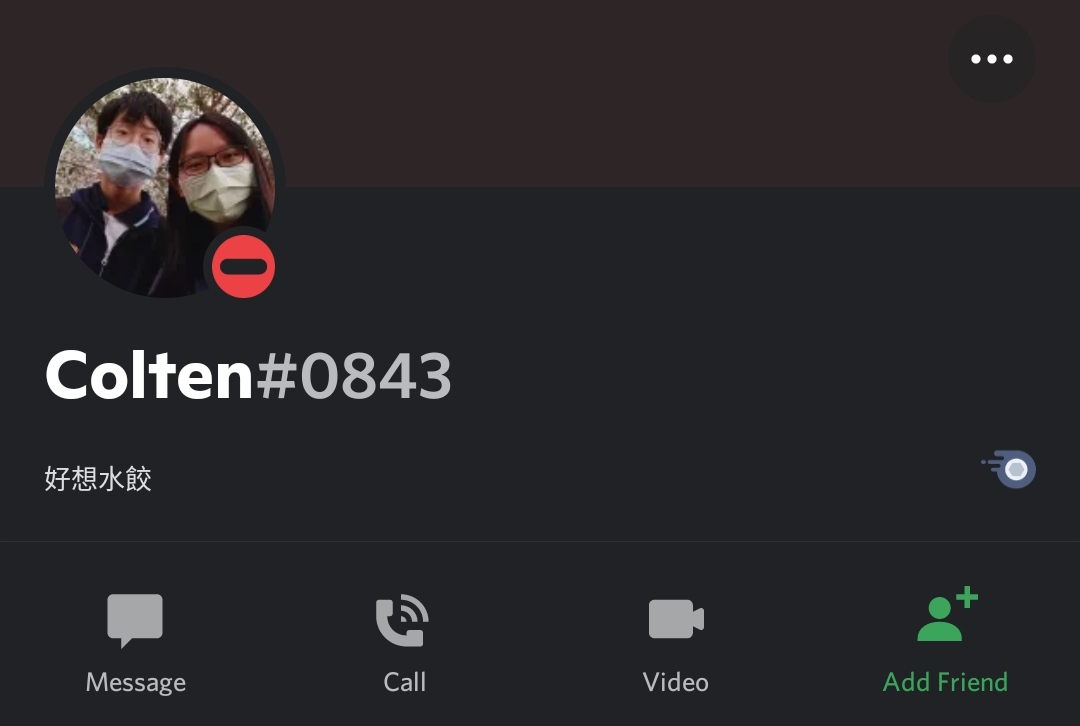
\includegraphics[height=0.5\textheight]{./src/Corzlten.png}
			\end{center}
		\end{itemize}
		
	\end{frame}

	\section{競賽先備知識}

	\section{題目中的雙標:時間複雜度與空間複雜度}

	\begin{frame}{什麼是時間複雜度}
		\begin{itemize}
			\item<1-> \sout{規劃考試作答時間嗎}
			\item<2-> 運算數量隨著資料量上升而上升的指數(函數)關係
			\item<3-> 用來估算這個程式在大資料量下的運算次數 (通常考慮最差情況)
			\item<4-> 與執行時間成正相關,但執行時間不是只受複雜度影響
			\item<5-> 用來判斷一個程式是否能達到題目要求
			\item<6-> 以大 O 符號 ($\mathcal{O(...)}$) 來表示
		\end{itemize}
	\end{frame}

	\begin{frame}{時間複雜度的算法}
		\begin{itemize}
			\item<1-> 以一次基本運算 (賦值、加法等等) 作為 $\mathcal{O}(1)$
			\item<2-> 計算每個函式或是迴圈會運行幾次基本運算
			\item<3-> 下圖是一個 $\mathcal{O}(n)$ 的程式
			\begin{center}
				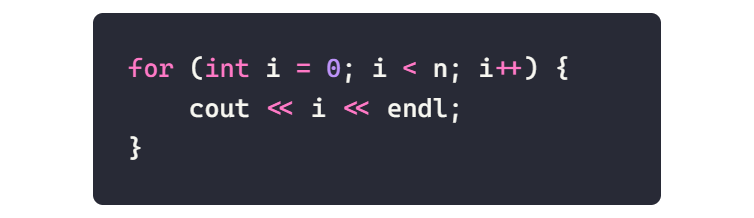
\includegraphics[width=1.0\textwidth]{./src/O(n)_1.png}
			\end{center}
		\end{itemize}


	\end{frame}

	\begin{frame}{時間複雜度的例子}
		\begin{center}
			請問這隻程式的時間複雜度是多少呢?
			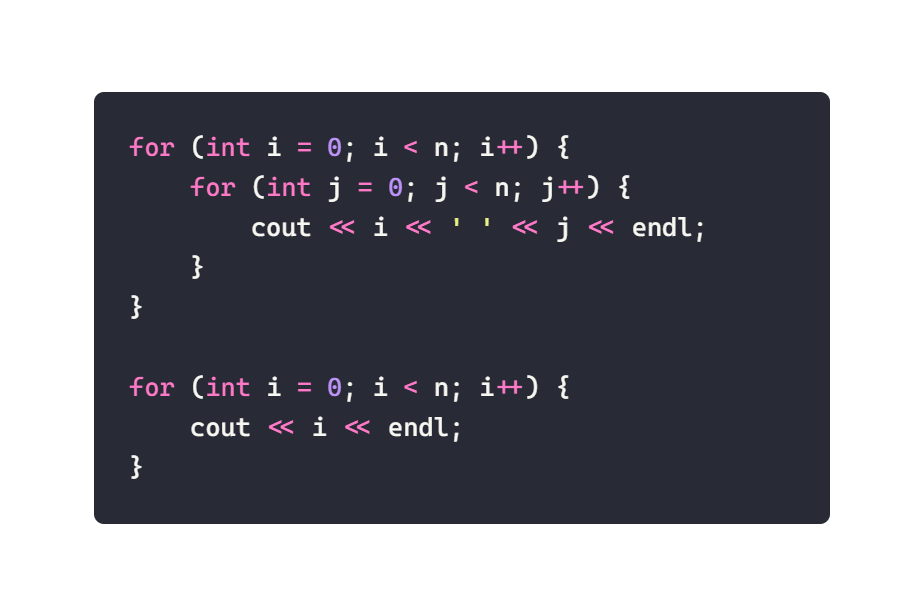
\includegraphics[height=0.9\textheight]{./src/O(n^2)_1.png}
		\end{center}
	\end{frame}

	\begin{frame}{時間複雜度的例子}
		\begin{itemize}
			\item<1-> 可能有些人覺得是 $\mathcal{O}(n^2+n)$
			\item<2-> 但實際上,當 $n$ 很大時,$\mathcal{O}(n)$ 對 $\mathcal{O}(n^2)$ 的影響微乎其微
			\item<3-> 量級差太多的項次我們會省略,並稱他為常數
			\item<4-> 因此這支程式的時間複雜度為 $\mathcal{O}(n^2)$
		\end{itemize}
	\end{frame}

	\begin{frame}{時間複雜度的例子}
		\begin{center}
			再來一個
		\end{center}
		\begin{center}
			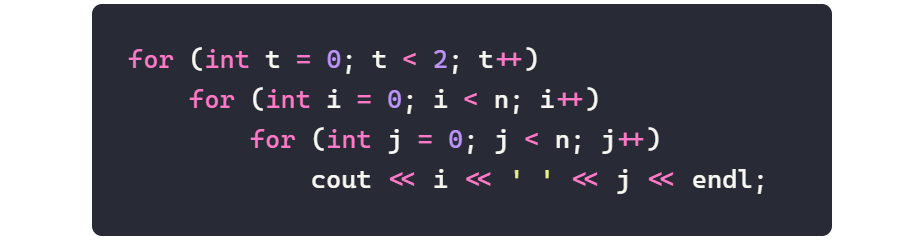
\includegraphics[height=0.4\textheight]{./src/O(n^2)_2.png}
		\end{center}
	\end{frame}

	\begin{frame}{時間複雜度的例子}
		\begin{itemize}
			\item<1-> $\mathcal{O}(2\times n^2)$ 還是 $\mathcal{O}(n^2)$?
			\item<2-> 我們仍然會將那個兩倍視為常數
			\item<3-> 為甚麼呢?
			\item<4-> 其實並不是所有的基本運算都是一樣的執行時間,像是 mod 就會比一般的加法還要慢,因此去計較是 $\mathcal{O}(2\times n^2)$ 還是 $\mathcal{O}(n^2)$ 是沒有意義的,能夠看出成長的趨勢即可
			\item<5-> 時間複雜度的計算,除了會忽略低次項之外,也會忽略係數
		\end{itemize}
	\end{frame}

	\begin{frame}{均攤時間複雜度}
		\begin{itemize}
			\item<1-> 我們在估算時間複雜度的時候,我們會以最壞的可能去估算,通常是考慮範圍最大的情況
			\item<2-> 但有些操作,在不同的數值所需的操作數可能大可能小,例如某個操作在 $i$ 為二的次方時的複雜度為 $\mathcal{O}(n)$,但在其他情況下的複雜度卻只有 $\mathcal{O}(1)$
			\item<3-> 那我們就可以將所有操作的複雜度加起來,再取平均,就會發現 $\mathcal{O}(n)$ 的情況被 $\mathcal{O}(1)$ 平攤掉了
			\item<4-> 這種有好有壞,對他做平均的分析方法就叫做均攤分析
		\end{itemize}
	\end{frame}

	\begin{frame}{一些常見的時間複雜度}
		\begin{itemize}
			\item $\mathcal{O}(1)$:基本運算
			\item $\mathcal{O}(n)$:線性搜、遍歷陣列
			\item $\mathcal{O}(n^2)$:氣泡排序、某些情況下的枚舉
			\item $\mathcal{O}(\log n)$:二分搜、快速冪
			\item $\mathcal{O}(n\log n)$:merge sort、某些分治演算法
				\begin{itemize}
					\item $\frac{n}{1}+\frac{n}{2}+\frac{n}{3}+...+\frac{n}{n}$ 也是 $\mathcal{O}(n \log n)$
				\end{itemize}
			\item $\mathcal{O}(n!)$:排列枚舉
			\item $\mathcal{O}(2^n)$:位元枚舉
		\end{itemize}
	\end{frame}

	\begin{frame}{時間複雜度的標準}
		\begin{itemize}
			\item<1-> 學會了如何估算時間複雜度之後,該怎麼判斷這個複雜度會不會過呢?
			\item<2-> 現在電腦處理器的運行時脈是以 GHz 的單位來表示的,代表了 CPU 一秒可以做 $n \times 10^9$ 次的基本操作
			\item<3-> 但是每一次的運算不會只需要一次的基本操作,再加上系統的效能分配,所以大概把他減去一個數量集,就可以得到 $10^8$ 這個數字
			\item<4-> 我們會以 $10^8$ 為標準,若時間複雜度算出來超過這個數字不少,那基本上就可以確定會得到 TLE
			\item<5-> Judge 的速度都不一樣,像是 Codeforces 就有機會跑到一秒接近 $10^9$,甚至有時候編譯器會幫我們做一些黑魔法加速,所以 $10^8$ 算是一個比較保守的估計
			\item<6-> 學會估算時間複雜度之後,有時候看到題目的範圍就可以大概猜出是什麼複雜度的解法
		\end{itemize}
	\end{frame}

	\begin{frame}{時間複雜度的優化}
		\begin{itemize}
			\item<1-> 接下來的課程,除了會教你如何成功地將答案算出來之外,也會教你如何優化這隻程式
			\item<2-> 所做的事情基本上就是在優化時間複雜度
			\item<3-> 這邊先舉一個最簡單的例子
		\end{itemize}
	\end{frame}

	\begin{frame}{前綴和優化}
		\begin{block}{TPR \#23 PH1 區間求和問題 (一維版本)}
			給定一個長度為 $N$ 的數列 $a$,接著有 $Q$ 筆查詢,對於每次查詢會輸入兩個變數 $L, R$ 代表要求 $[L, R]$ 之間的元素和,也就是 $\sum_{i=L}^{R}{a_i}$\\
			$(n \le 2 \times 10^5, Q \le 10^4)$
		\end{block}

		\begin{itemize}
			\item<2-> 先簡單計算一下暴力解的時間複雜度
			\item<3-> 每次查詢最多會計算 $N$ 個元素,共查詢 $Q$ 次,所以時間複雜度是 $\mathcal{O}(NQ)$,顯然會 TLE
			\item<4-> 我們會發現到說,在這 $Q$ 次的操作中,我們可能會重複計算到很多重疊的區間,例如我們如果已經算過 $[1, 10]$,那再算 $[2, 5]$ 時就重複計算到了區間
			\item<5-> 那我們還不如預先將一些區間先算出來,後面要用就直接用
			\item<6-> 我們可以定義 $pre_i$ 是 $1 \sim i$ 的前綴和,也就是 $\sum_{j=1}^{i}{a_j}$,那如果要取得 $[l, r]$ 的和,就只需要算 $pre_r - pre_{l-1}$ 就可以了
			\item<7-> 這個就是最常見的\textbf{前綴和優化},而利用區間相減得到另外一個區間的動作就叫做\textbf{差分}
		\end{itemize}
	\end{frame}

	\section{先備知識與實用技巧}

	\begin{frame}{常見的數學符號}
		\begin{itemize}
			\item $\sum$ 代表連加,如 $\displaystyle\sum_{i=1}^{n}{a_i}$ 代表將 $a_1 \sim a_n$ 加起來
			\item $\prod$ 則是將 $\sum$ 的連加變為連乘
			\item $a \mid b$ 代表 $a$ 整除 $b$ 或是 $b$ 能被 $a$ 整除例如 $6 \mid 24$
			\item $\gcd(a, b)$ 代表 $a,b$ 的最大公因數
			\item $lcm(a, b)$ 代表 $a,b$ 的最小公倍數
			\item $log_a{b}$ 代表 $a^{log_a{b}} = b$,而電腦科學中的 $\log$ 是以 $2$ 為底的 $(\log_2{b})$
				\begin{itemize}
					\item $\log_2{8}=3$,$\log_2{\frac{1}{2}}=-1$
				\end{itemize}
			\item $a\mod{b}$ 代表 $a$ 對 $b$ 取餘數的結果
		\end{itemize}
	\end{frame}

	\begin{frame}{位元運算}
		\begin{itemize}
			\item<1-> AND: 在 C++ 中以 \& 表示,當兩個 bit 都為 $1$ 時為 $1$,否則為 $0$
			\item<2-> OR: 在 C++ 中以 $\mid$ 表示,當兩個 bit 有至少一個為 $1$ 時為 $1$,否則為 $0$
			\item<3-> XOR: 在 C++ 中以 $\ \^$ 表示,當兩個 bit 洽有一個為 $1$ 時為 $1$,否則為 $0$
			\item<4-> NOT: 在 C++ 中以 $\ \~$ 表示,代表將 $0$ 轉為 $1$,$1$ 轉為 $0$
		\end{itemize}
	\end{frame}

	\begin{frame}{萬用標頭檔}
		\begin{itemize}
			\item<1-> 在 C++ 中,有這麼一個標頭檔叫做 bits/stdc++.h
			\item<2-> 他會函入幾乎所有常用的標頭檔
			\item<3-> 這個標頭檔是方便用,但還是盡量要知道每個容器或是函式需要含入的標頭檔是哪個
			\item<3-> 請別在刷題以外的地方使用
			\item<4-> 接下來兩個禮拜的內容,講師的範例程式碼應該超過九成都是使用萬用標頭檔
		\end{itemize}
	\end{frame}

	\begin{frame}{IO 加速}
		\begin{itemize}
			\item<1-> 若是使用 cin, cout 來輸入輸出,會發現他的速度比 scanf, printf 還要慢上不少
			\item<2-> 這是因為 cin 會自動將緩衝區清除,而 scanf 不會
			\item<3-> 緩衝區清除的用意是讓使用者可以馬上看到輸入的文字
			\item<4-> 但這對於演算法題目並不是非常必要
			\item<5-> 因此我們可以使用 cin.tie(0) 來解除自動清除緩衝區
			\item<6-> 需要注意的是,endl 也會清除緩衝區,需要將 endl 換成 '$\backslash$n' 才能夠有效的加速
			\item<7-> 另外,為了避免使用者與 scanf, printf 混用,C++ 會自動將兩種輸入方式同步,這也會造成延遲,但我們如果不會混用的話,就可以將其解除
			\item<8-> 解除方法: \text{ios::sync\_with\_stdio(0);}
		\end{itemize}
	\end{frame}

	\begin{frame}{define}
		你可能會在一些選手的程式碼看到這種東西:
		\begin{center}
			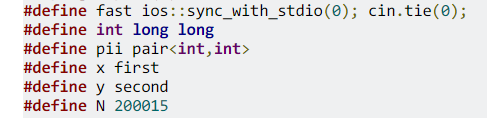
\includegraphics[width=0.5\textwidth]{src/victorgao_define.png}
		\end{center}

		\begin{itemize}
			\item<1-> 這是 C++ 的好用功能
			\item<1-> 可以將 A define 成 B
			\item<2-> 舉例:\#define int long long
			\item<3-> 可以有效的加快寫題的過程
			\item<4-> 講師們的範例程式碼許多都有將 int define 成 long long,自己在練習時要注意溢位的問題
		\end{itemize}
	\end{frame}

	\begin{frame}{全域變數}
		\begin{itemize}
			\item<1-> 其實區域變數是有大小限制的
			\item<2-> 因此若是建了一個比較大的表,就有可能會造成 RE (Runtime Error)
			\item<3-> 將一些系統輸入的變數、陣列或是額外建的表、資料結構等宣告在全域,就能夠避免空間太大而產生 RE 的情況
			\item<4-> 這在開發上可能是個不好的習慣,因此要用對地方
		\end{itemize}
	\end{frame}

	\begin{frame}{pass by reference}
		\begin{itemize}
			\item<1-> 在一般的函數傳遞上,例如 f(a),我們只是將一個值傳過去而已,這稱為 pass by value,若是在 f() 內更改 a,呼叫地的 a 是不會有變化的
			\item<2-> 但如果我們想要能夠直接改到原本的值,就可以使用這個語法,可以想像成是他會將原始的東西傳過去,所以在更改的時候就是直接改呼叫地的值
			\item<3-> 在使用上,我們只需在函式宣告傳入值的變數前方加上一個 \&,就可以成功達成 pass by reference
		\end{itemize}
	\end{frame}

	\begin{frame}{pass by reference}
		\begin{center}
			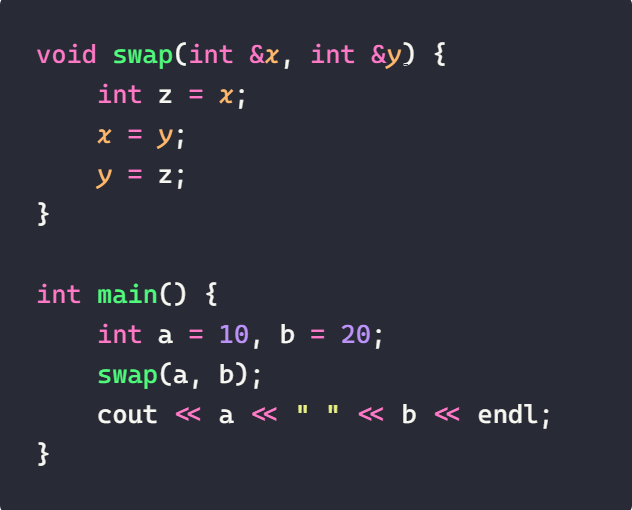
\includegraphics[width=0.5\textwidth]{./src/call_by_reference_swap.png}
		\end{center}
		\begin{center}
			這個程式碼會輸出 $20\ 10$
		\end{center}
	\end{frame}

	\begin{frame}{range based for loop}
		\begin{itemize}
			\item<1-> 寫過一些高階語言的話,可能會看到一些 forEach 或是 for...in... 之類的迴圈
			\item<2-> C++11 也加入了類似這種功能的語法,稱為 range based for loop
			\item<3-> 如果我有一個整數陣列 arr,那麼我只要呼叫 for (int it: arr),那麼他就會自動遍歷 arr 中的每個元素,並以 it 這個變數呈現
			\begin{center}
				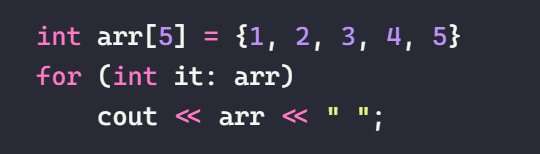
\includegraphics[width=0.6\textwidth]{./src/range_based_for_loop_1.png}\\
				output: 1 2 3 4 5
			\end{center}
		\end{itemize}

	\end{frame}

	\begin{frame}{range based for loop with auto}
		\begin{itemize}
			\item<1-> 如果我今天是一個 struct 陣列,而這個 struct 的名字很長,不想打那麼長怎麼辦?
			\item<2-> 在 C++14 中,新增了 auto 這個語法,當有明確的初始值,auto 就會自動判斷它的型態並轉換成他
			\item<3-> 所以我們可以直接使用 for (auto it: arr) 就可以完成整個陣列的遍歷了
			\begin{center}
				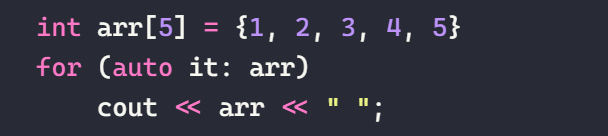
\includegraphics[width=0.6\textwidth]{./src/range_based_for_loop_2.png}\\
				output: 1 2 3 4 5
			\end{center}
		\end{itemize}
	\end{frame}

	\begin{frame}{range based for loop with reference}
		\begin{itemize}
			\item 然後你會發現,剛剛的寫法是 pass by value 的,沒有辦法更改到陣列中的內容
			\item 那我們就把他變成 pass by reference 就好啦
			\begin{center}
				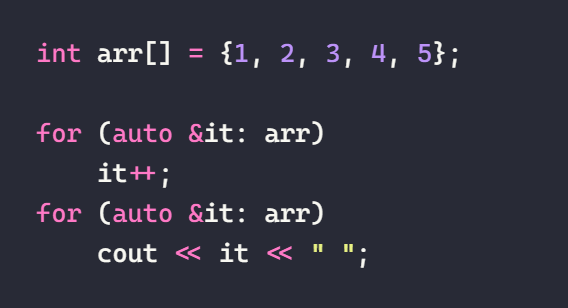
\includegraphics[width=0.5\textwidth]{./src/range_based_for_loop_3.png}\\
				output: 2 3 4 5 6
			\end{center}
		\end{itemize}
	\end{frame}

	\begin{frame}{sort}
		\begin{itemize}
			\item<1-> 當大家在寫 sort 的 compare 函式時,大概會寫一個 return a < b 之類的東西
			\item<2-> 那如果寫的是 a $\le$ b 呢?
			\item<3-> 如果你有一個長度足夠大、且每個元素都相同的陣列,並且在 compare 函式裡嘗試輸出每次傳入的值,你會發現他進入了無窮迴圈
			\item<4-> 為甚麼呢?
			\item<5-> 嘗試在本機運行以下的程式
			\begin{center}
				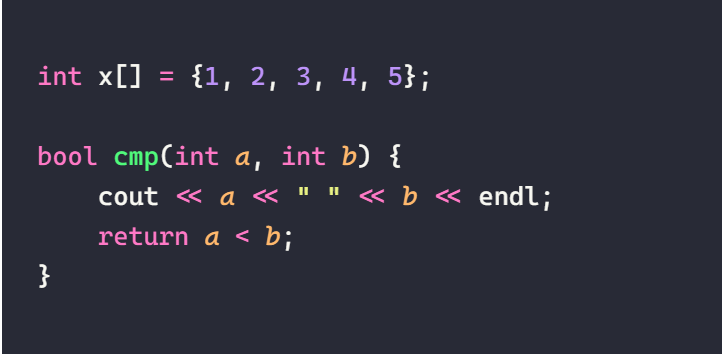
\includegraphics[width=0.5\textwidth]{./src/compare_1.png}\\
			\end{center} 
		\end{itemize}
	\end{frame}

	\begin{frame}{sort}
		\begin{itemize}
			\item<1-> 你會發現到,$a, b$ 的前後順序竟然是相反的
			\item<2-> 這是因為,sort 他會先預設你要交換,然後再問你這樣對不對,如果不對 (false) 就換回原本的順序
			\item<3-> 如果你是用 $\le$ 的話,遇到有相同的元素,系統每次詢問時你都跟他說這樣對,他就會一直換一直換,最後就會得到 RE
			\item<4-> 因此 compare 函式是不能使用 $\le$ 或是 $\ge$ 的
		\end{itemize}
	\end{frame}

	\begin{frame}{lambda}
		\begin{itemize}
			\item<1-> 覺得每次 sort 都要寫 compare 函式很麻煩嗎?
			\item<2-> C++14 提供了匿名函式 lambda 可以直接內嵌在 sort 呼叫裡
			\item<3-> lambda 的用法非常多元,以下只展示最簡易的用法\\
			\begin{center}
				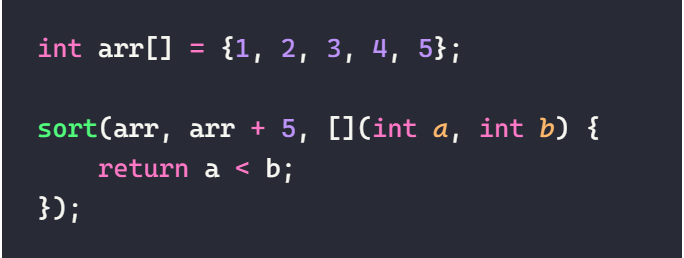
\includegraphics[width=0.5\textwidth]{./src/lambda_1.png}
			\end{center}
		\end{itemize}
	\end{frame}

	\begin{frame}{自訂 operator}
		\begin{itemize}
			\item<1-> 有時候我們自定義了一個 struct,並且想要讓他可以做一些相加的操作,我們可能會寫一個函式
			\item<2-> 但是要呼叫一個函式看起來就不漂亮
			\item<3-> 所以我們可以自定義一個運算子,如此一來只要直接呼叫 A+B 就行了
			\item<4-> 用法一樣超多,舉個簡單的例子
			\begin{center}
				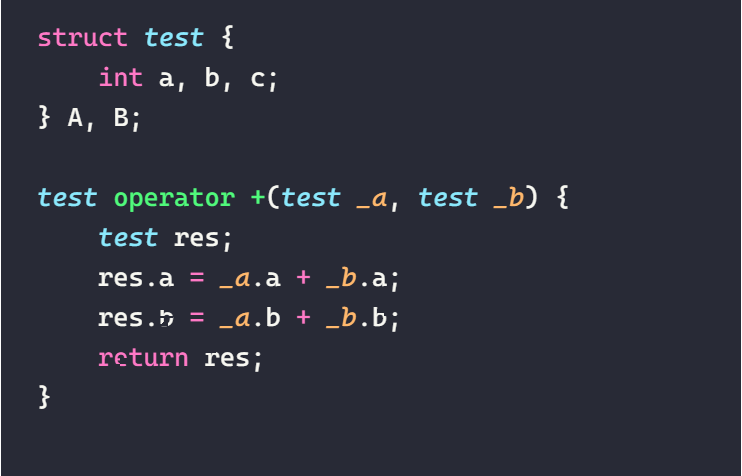
\includegraphics[height=0.5\textheight]{src/operator_1.png}\\
			\end{center}
		\end{itemize}
	\end{frame}

	\begin{frame}{stringstream}
		\begin{itemize}
			\item<1-> 如果今天有未知的數字,該怎麼輸入呢?
			\item<2-> 我們可能會用個 getline 將整行讀進來,然後再呼叫函數將字串轉換為多個數字
			\item<3-> 但其實 C++ 有內建工具:字串串流 (stringstream),使用需 include sstream
			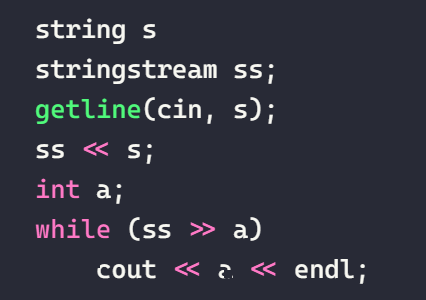
\includegraphics[height=0.3\textheight]{./src/sstream_1.png}
			\item<4-> 如此一來就可以將字串中的所有數字取出了
		\end{itemize}
	\end{frame}

	\begin{frame}{編譯器對執行時間的影響}
		\begin{itemize}
			\item<1-> 相信大家在一些 OJ 提交程式碼時都會看到一串編譯的指令,這對執行結果有什麼關係呢?
			\item<2-> 其實編譯器的參數會大大影響到執行的時間
			\item<3-> 例如更新的版本可能會將你的程式碼更加優化
			\begin{itemize}
				\item<4-> C++20 > C++17 > C++14
			\end{itemize}
			\item<5-> 裁判機是以 32-bit 運行或是 64-bit 運行也是有影響的,位元數越高代表電腦可以同時處理越多事情
			\begin{itemize}
				\item<6-> 以 Codeforces 為例:GNU G++20 11.2.0 (64 bit, winlibs) > 	GNU G++17 7.3.0					
			\end{itemize}
			\item<7-> 編譯器優化也有影響
			\begin{itemize}
				\item<8-> 以 O2 優化為例,他就會自動把你的程式碼做優化,讓他省去一些不必要的動作
				\item<8-> 可以上 https://godbolt.org/ 這個網站嘗試,他會將你的 Code 轉成較接近機器可讀的組合語言 (assembly)
			\end{itemize}
		\end{itemize}
	\end{frame}

	\section{總結}

	\begin{frame}{總結}
		\begin{itemize}
			\item 這堂課教到了許多演算法競賽的入門知識,有些是必要的,有些是非必要的,希望學員們能夠學到一些小技巧
			\item 希望學員們能夠對演算法競賽有更多的認識
			\item 演算法競賽中的某些習慣或是技巧並不是在每個地方都適合使用的,接下來的課程會教到更多高深技巧,這些都只是工具,希望大家都可以用在適合的地方,不要在不適合的地方使用
		\end{itemize}
	\end{frame}
\end{document}